\documentclass[sigconf]{acmart}

\usepackage{booktabs} % For formal tables

% Copyright
%\setcopyright{none}
%\setcopyright{acmcopyright}
%\setcopyright{acmlicensed}
\setcopyright{rightsretained}
%\setcopyright{usgov}
%\setcopyright{usgovmixed}
%\setcopyright{cagov}
%\setcopyright{cagovmixed}

% DOI
\acmDOI{10.475/123_4}

% ISBN
\acmISBN{123-4567-24-567/08/06}

%Conference
\acmConference[ACM ICMR2017]{Multimedia Forensics and Security Workshop}{June 2017 }{Bucharest, Romania} 
\acmYear{2017}
\copyrightyear{2017}

%\acmPrice{15.00}

\graphicspath{{./images/}}
\usepackage{listings}
\usepackage{url}
\usepackage{tabularx}
\usepackage{booktabs}
\usepackage{stfloats}

%%%% Bullets inside table %%%%
\newcommand{\tabitem}{~~\llap{\textbullet}~~}

%%%%%%%%% JSON BEGIN %%%%%
\usepackage{xcolor}
\colorlet{punct}{red!60!black}
\definecolor{background}{HTML}{EEEEEE}
\definecolor{delim}{RGB}{20,105,176}
\colorlet{numb}{magenta!60!black}

\lstdefinelanguage{json}{
	basicstyle=\normalfont\ttfamily,
	numbers=left,
	numberstyle=\scriptsize,
	stepnumber=1,
	numbersep=8pt,
	showstringspaces=false,
	breaklines=true,
	frame=lines,
	backgroundcolor=\color{background},
	literate=
	*{0}{{{\color{numb}0}}}{1}
	{1}{{{\color{numb}1}}}{1}
	{2}{{{\color{numb}2}}}{1}
	{3}{{{\color{numb}3}}}{1}
	{4}{{{\color{numb}4}}}{1}
	{5}{{{\color{numb}5}}}{1}
	{6}{{{\color{numb}6}}}{1}
	{7}{{{\color{numb}7}}}{1}
	{8}{{{\color{numb}8}}}{1}
	{9}{{{\color{numb}9}}}{1}
	{:}{{{\color{punct}{:}}}}{1}
	{,}{{{\color{punct}{,}}}}{1}
	{\{}{{{\color{delim}{\{}}}}{1}
	{\}}{{{\color{delim}{\}}}}}{1}
	{[}{{{\color{delim}{[}}}}{1}
	{]}{{{\color{delim}{]}}}}{1},
}
%%%%%%%%%%%%%%%%%%%%JSON END %%%%



\begin{document}
\title[Automatic Large Scale Image Forensics]{An Approach for Automatic and Large Scale Image Forensics and Search}
\author{Thamme Gowda\textsuperscript{1}, Kyle Hundman\textsuperscript{2}, Chris A. Mattmann\textsuperscript{1,2}}
\email{thammegowda.n@usc.edu}
\affiliation{\begin{tabular}{*{2}{>{\centering}p{.45\textwidth}}}\textsuperscript{1}Computer Science Department & \textsuperscript{2}Jet Propulsion Laboratory \tabularnewline University of Southern California & California Institute of Technology \tabularnewline Los Angeles, CA 90089 USA & Pasadena, CA 91109 USA \end{tabular}}

% The default list of authors is too long for headers}
\renewcommand{\shortauthors}{T. Gowda, K. Hundman, C. Mattmann}

%\titlenote{Apache Tika is a open source project hosted on Apache Software Foundation and Tensorflow is another opensource framework for deeplearning}
%\subtitle{Memex program}
%\%subtitlenote{Credits to DARPA Memex}


% The default list of authors is too long for headers}
%\renewcommand{\shortauthors}{T. Gowda and C. Mattmann}


\begin{abstract}
This paper describes uses of image recognition in content analysis, methods of integration and associated challenges and our final architecture of the system. //TODO: write this later as a summary of paper...
\end{abstract}

%
% The code below should be generated by the tool at
% http://dl.acm.org/ccs.cfm
% Please copy and paste the code instead of the example below. 
%
\begin{CCSXML}
<ccs2012>
<concept>
<concept_id>10002951.10003317</concept_id>
<concept_desc>Information systems~Information retrieval</concept_desc>
<concept_significance>500</concept_significance>
</concept>
<concept>
<concept_id>10002951.10003317.10003371.10003386.10003387</concept_id>
<concept_desc>Information systems~Image search</concept_desc>
<concept_significance>500</concept_significance>
</concept>
<concept>
<concept_id>10010405.10010462</concept_id>
<concept_desc>Applied computing~Computer forensics</concept_desc>
<concept_significance>300</concept_significance>
</concept>
</ccs2012>
\end{CCSXML}

\ccsdesc[500]{Information systems~Information retrieval}
\ccsdesc[500]{Information systems~Image search}
\ccsdesc[300]{Applied computing~Computer forensics}

% We no longer use \terms command
%\terms{Theory}

\keywords{Image Recognition, Multimedia Forensics, Information Retrieval}

\maketitle

\section{INTRODUCTION}
%% TODO: introduce Content Analysis and role in DARPA MEMEX
Over the past two years, our research team has borne witness to the ease and availability of potentially criminal goods and services on the modern Internet. In particular, our team's work on the DARPA Memex project has focused on the issues of online gun sales, as such sales can have grim consequences in that they provide a medium for buyers and sellers to circumvent traditional background checks. In turn, this proliferates the sale of dangerous semi-automatic weapons and can lead directly to loss of human life. For instance, a New York Police Department (NYPD) investigation in 2013 identified guns used in one suicide and four murders and traced their origin to transactions on the website \url{armslist.com}\cite{raja_2016}. 

The ability to rapidly detect and analyze gun sales transactions is a significant challenge. There are hundreds of both national and regional gun sales sites like Armslist, \url{floridaguntrader.com}, or \url{gunbroker.com}. Besides the sheer number of sites, many of the sites share common themes indicative of today's {\em Deep} web. They require a login to either buy or sell, making bulk analysis difficult for traditional web crawlers. A significant number of the sites use Ajax or Javascript for pagination, or for displaying gun images from an ad; this also makes automatic analysis a challenge. But most significantly, the actual content required to determine the answers to significant questions regarding these weapons (``is this an automatic weapon?'', ``is this a long or a short gun?'', ``are there multiple weapons being sold?'') are the {\em images} of the weapons themselves. 

We have previously worked on bulk image analysis from the deep web as it relates to human trafficking data \cite{mattmann7tg} using the Apache Tika content detection and analysis framework \cite{mattmann2011tika}. Our work there focused on image metadata forensics as an alternative to image pixel based analyses and object detection and recognition. Though metadata forensics were promising in human trafficking, weapons required pixel-based analyses. Based on our study of over 80 websites and online forums that specialize in the exchange of weapons, object recognition and computer vision were needed to automatically discern whether or not the guns being sold are automatic or semi-automatic, whether they have been stolen (using serial-number identification), and whether the transactions are potentially illegal. Automatically being able to discern these types of object properties in bulk analyses of image data has the potential to thwart crimes and, ultimately, to save lives.

Law enforcement agencies do not have the manpower to effectively monitor the scale of weapons ads on the aforementioned sites and forums and though the ads, like the whole Internet, contain a large amount of text \cite{mphillips-EOT2012}, the proliferation of images necessitates object recognition and image analysis at scale. Our recent work in DARPA's MEMEX initiative has focused on expanding Apache Tika to support such analysis.

Historically, the best object recognition systems were inaccurate, but this has changed due to recent advancements in deep neural networks, larger training datasets, and improved computing resources. Tensorflow is a scalable, Python-based system and it natively supports image recognition via its \em {Inception} model \cite{abadi2016tensorflow}. \em{Inception} provides a neural network trained on the ImageNet corpus \cite{krizhevsky2012imagenet}, a dataset of 14,197,122 images classified using text from the WordNet taxonomy. The end result is a highly-scalable off-the-shelf system that can accurately identify and classify objects in images into a thousand categories. Combining this capability with Apache Tika's native support for detecting thousands of file formats, extracting their metadata and textual content, is an attractive, automated solution that can perform bulk analysis in the weapons domain, but more generally, in any context where text and images are present and such analyses are required.

Integration of Tensorflow with Tika presented a significant challenge: Tensorflow does not provide out of the box bindings to Java based frameworks. Apache Tika is primarily written in Java and thus integrating with Tensorflow is not straight forward like any other JVM compatible libraries. Our research directly addresses this and contributes several methods that make Tensorflow easier to integrate into Java-based systems like Tika, and any digital forensics system that can make a call to an application programming interface (API). In this paper, we report on our integration of Tika and Tensorflow using the Weapons domain as a motivating example. We evaluate the integration in both its robustness in objection recognition with zero training beyond that of ImageNet and demonstrate that Tensorflow and Tika are a scalable forensics solution for bulk image analysis on the Deep Web.

The remainder of this paper is organized as follows. Section 2 discusses the collection of the Weapons dataset and its properties. Section 3 presents our integration of Tika and Tensorflow via three methods: (1) command line invocation; (2) Google's RPC (gRPC) integration; and (3) Representational Entity State Transfer (REST) \cite{Fielding:2000:ASD:932295} integration. Section 4 qualitatively evaluates our integration techniques and quantitatively evaluates the efficacy of Tensorflow, ImageNet and Tika-based image forensics. Section 5 rounds out the paper.

\begin{figure*}
	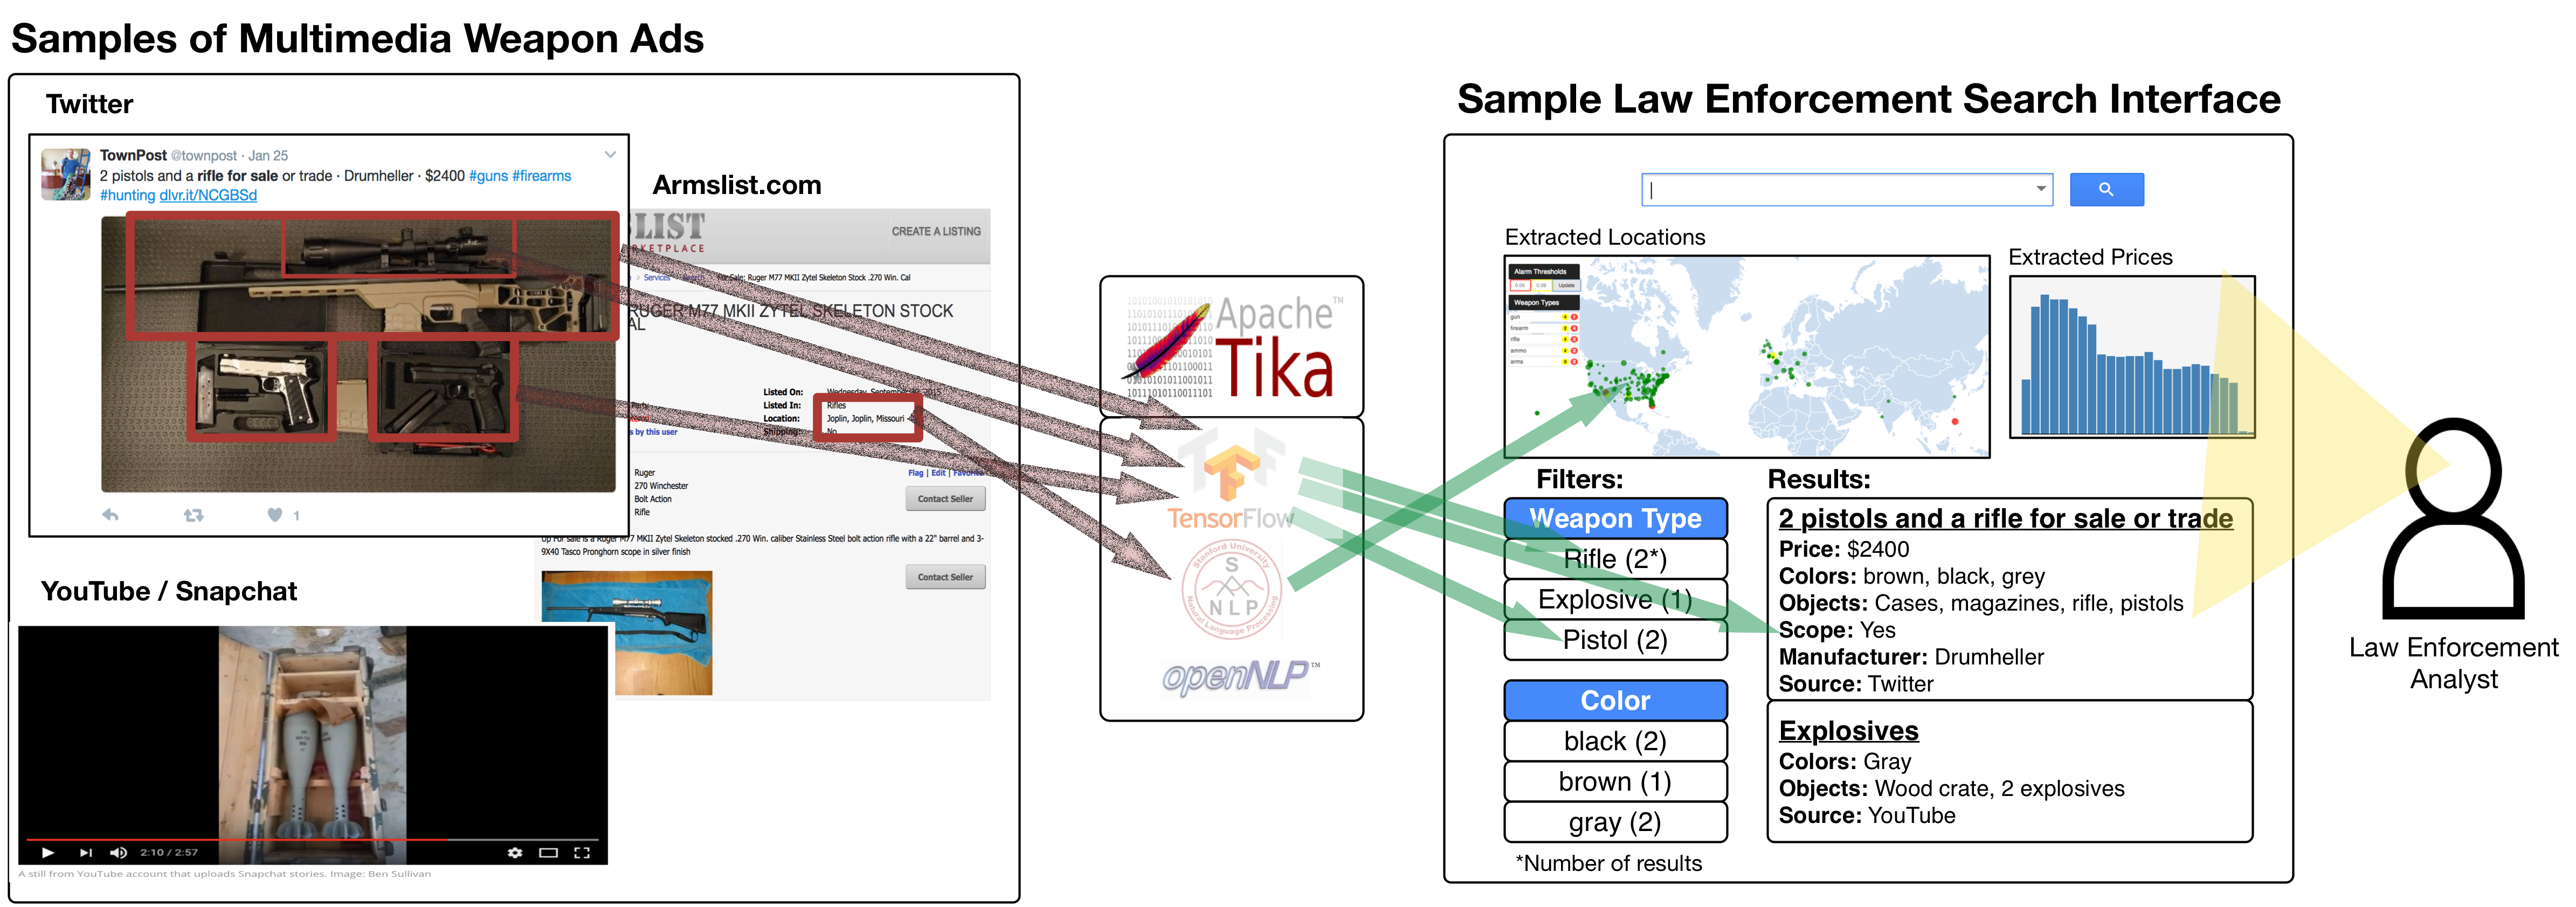
\includegraphics[width=\textwidth,height=6cm]{interface-diagram}
	\caption{This diagram demonstrates how the integration of Tika and Tensorflow facilitates interfaces in-depth search across heterogenuous content types. There are several extensions to our object recognition implementation as well, including more refined categories, optical-character recognition, and image similarity metrics.}
	\label{fig:interface-diagram}
\end{figure*}

\section{CONTENT ANALYSIS IN MEMEX PROGRAM} \label{sec:memex}
This section discusses the background and motivations of DARPA Memex program and its datasets. The current commercial web search engines provides a generalized search interface to all users~\cite{}. However, in the context of cyber security, the commercial search engines miss resources from the deep and dark web which are essential for law keeping agencies. The goal of Memex program is to develop softwares that can quickly and thoroughly organize and search subsets of information relevant to the individual interests. The first two interests were in the domains of human trafficking and illegal weapon sale.

\subsection{Data Collection}
\label{sec:memex-datacollection}
Several web crawlers were used to discover and retrieve information from the websites.
Along with the general purpose web crawlers, there were specialized crawler for the retrieval of dark data using TOR protocol \cite{} and also specialized in retrieval of dynamic AJAX content guarded by login forms. The fetched data were cached within the system for analysis due to the ephemeral nature of the content at the sources.

\subsection{Memex Dataset} \label{sec:memex-dataset}
The dataset used in our experiment was a subset of memex dataset in public domain. It contained 7.2 million documents in the illegal weapon sales domain in which 1.4 documents were images. We had analyzed the textual documents and the named entities separately in a different experiment using named entity recognition models and extractors for people, location, organization, weapon-name and weapon-types. In this experiment we were interested in labeling images by classifying them into various classes. Usually web crawlers fetches all resources linked in the web pages and hences classification was an important pre-processing to remove noise for the later analysis.

\subsection{Tools for Law Enforcement} \label{sec:memex-tools}
The ultimate goal of integrating diverse content scattered across the web is to provide law enforcement analysts with tools that will help them quickly identify relevant information. In the context of Memex, multimedia content is essential in helping analysts sift through millions of ads in search of illicit sales; images and videos often provide salient information not available in text. In many cases, illegal weapons dealers intentionally embed revealing details in rich content mediums because they are harder to identify. This thinking coincides with the rise of weapons trafficking on social media platforms such as Snapchat, YouTube, and Instagram, where communication is centered around images and video \cite{socialmedia}. The integration of Tensorflow and Tika provides a single, streamlined platform that unites the extraction of textual and rich content. This combined content can then be exposed through search and visualization interfaces that improve analysts' abilities to drill-down and explore comprehensive, diverse content contained in weapons ads (see Figure). Our use of Tensorflow and the Inception-V3 model serves as an example of the benefits of this integration and the types of insights and capabilities it facilitates in the future. 
%\section{OBJECT RECOGNITION} \label{sec:obj-rec}

\subsection{Deep Learning } \label{sec:deeplearning-imagenet}
\subsection{ImageNet} \label{sec:imagenet}

\subsection{Inception Network } \label{sec:inceptionnet}

\section{INTEGRATION} \label{sec:integration}
We defined an interface named \texttt{ObjectRecogniser} to facilitate multiple implementation of object recognizer. The image recognition framework was developed for the \texttt{ObjectRecogniser} contract. The main part of this contract is a function that accepts image data and returns list of \texttt{RecognisedObject}s

%% TODO: Summarize the challenges
%% TODO: List the available methods
The following methods of integration were investigated in the order of listing:
\begin{itemize}
\item Command Line Invocation
\item Java Native Interface
\item gRPC Remote Procedure Calls
\item Representational State Transfer API
\end{itemize}

\begin{figure*}
	\includegraphics[width=\textwidth,height=5cm]{tensorflow-tika-integration}
	\caption{Tika and Tensorflow Integration}
	\label{fig:tf-tika-integration}
\end{figure*}

%% 1. CLI
\subsection{Command Line Invocation (CLI)} \label{sec:int-cli}
Command Line Invocation is the most simple way of integration. We created a python based CLI tool as an entry point to tensorflow's image recognition network. This tool inspected the environment for its requirements. When its requirements were not met it simply failed by reporting the failure. Some of its requirements were:
\begin{enumerate}
\item NumPy
\item TensorFlow
\item Transitive dependencies of TensorFlow
\item Inception Net Model
\end{enumerate}
Apache Tika executed in the JVM process where as on every invocation of CLI tool, a new native process was created and destroyed. Tika passed image path as command line argument to the tool as shown in Figure \ref{fig:tf-tika-integration} (a). The tool parsed the arguments, then passed the content to tensorflow network and reported the results by printing it to standard output. Tika parser then read the result from its output stream. The pros and cons are described in the Section \ref{sec:eval-cli}
%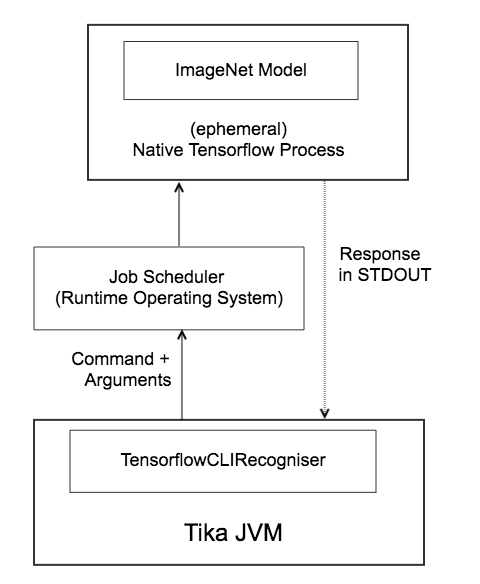
\includegraphics[scale=0.40]{tika-tflow-cli-design}

%% 2. JNI
\subsection{Java Native Interface (JNI)} \label{sec:int-jni}
The next approach we investigated was the Java Native Interface (JNI). JNI is the vendors' recommended way of integrating native code libraries to Java frameworks\cite{}. JNI acts as glue between bytecode instructions that runs within Java Virtual Machine (JVM) and the native  code instructions that runs directly on the CPU. Theoretically, this is the best way of merging JVM world with the native code\cite{}. At runtime, the bytecode of Tika (caller) and native code of tensorflow (callee) runs within the single process from the operating system's perspective as shown in Figure \ref{fig:tf-tika-integration} (b).

%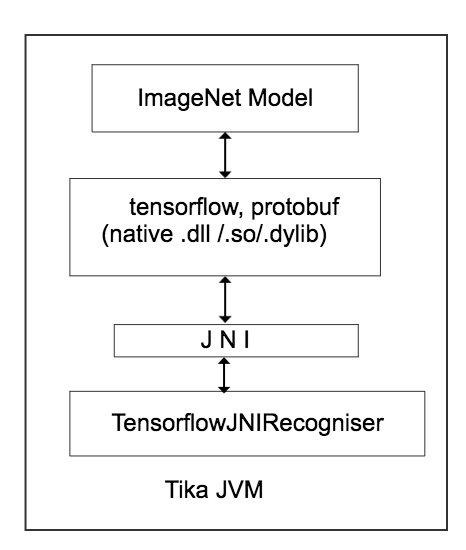
\includegraphics[scale=0.40]{tika-tflow-jni-design}

%% 3. RPC
\subsection{gRPC Remote Procedure Calls (gRPC)} \label{sec:int-rpc}
The developers of Tensorflow framework recommended to use gRPC based integration for the production systems\cite{goog-tfserve}. gRPC is a client-server based architecture in which caller acts as a RPC client and callee serves as a server in a different address space. Unlike traditional RPC frameworks, gRPC is a high performance, CPU and bandwidth efficient transport on top of HTTP/2 that supports full duplex streaming\cite{about-grpc}. In our case, we embedded gRPC client in Tika JVM and exported Tensorflow image recognition capabilities as remote procedures via gRPC service. We used Tensorflow Serving, a gRPC server implemented in C++, and also created a docker container to host it.

%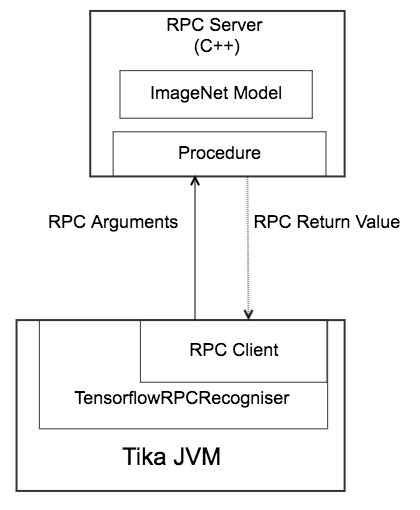
\includegraphics[scale=0.40]{tika-tflow-RPC-design}

%% 4. REST
\subsection{Representational State Transfer (REST) Application Programming Interface (API)} \label{sec:int-rest}
Representation State Transfer (REST) is a popular client-server architecture paradigm for connecting heterogeneous systems without the need of states\cite[Chapter~5]{Fielding:2000:ASD:932295}. The REST application programming interfaces (API) is powered by an HyperText Transfer Protocol (HTTP) which abstracts the complexities of Transmission Control Protocol.
We crated REST API for tensorflow image recognition using python Flask\cite{}. The Flask based HTTP service registered a TCP port and offered HTTP API end points as shown in Figure \ref{fig:tf-tika-integration} (d).
An API end point accepted HTTP POST requests with image data in the multi-part-form body. This service loaded the InceptionV3Net \cite{SzegedyVISW15} model during the initialization phase and held the model in memory for reusing it during the future HTTP Requests.

% \begin{figure}[h]
%     \centering
%     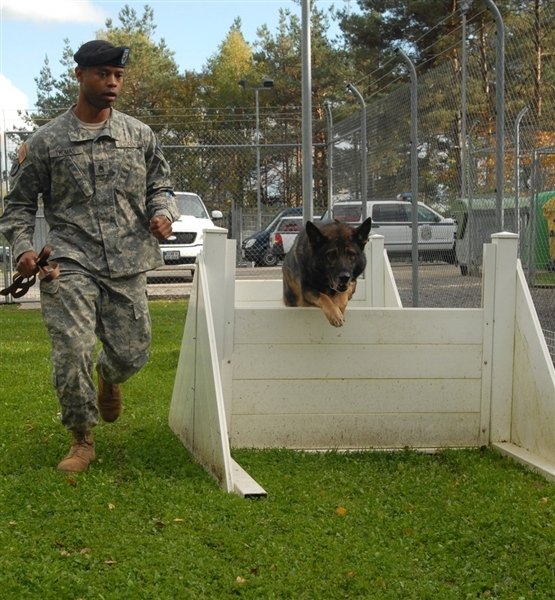
\includegraphics[width=\columnwidth]{military_dog}
%     \caption{Military Person with a German Shepherd Dog \newline Courtesy: Wikimedia Commons}
%     \label{fig:military-dog}
% \end{figure}

% The REST API, upon recognizing the objects in the image \ref{fig:military-dog}, returned the response in the JSON format with the following structure:

% \begin{lstlisting}[language=json, label=code:json-output,
% 	frame=single, xleftmargin=5.0pt, xrightmargin=5.0pt,
%     caption=JSON Response from REST API]
% {
%   "confidence": [ 0.362026, 0.130613],
%   "classnames": [
%     "German shepherd, alsatian",
%     "military uniform"
%   ],
%   "classids": [211, 866 ],
%   "time": {
%     "read": 1,
%     "units": "ms",
%     "classification": 257
%   }
% }
% \end{lstlisting}

On the other side of the system, we implemented the class \texttt{TensorflowRESTRecogniser} which used HTTP Client to communicate with REST API. This implementation of \texttt{ObjectRecogniser} converted the image data to HTTP POST request with multipart form data and sent it to REST API. It parsed the JSON response to retrieve the object names, ids and confidence scores. We also created a docker specification for bootstrapping the tensorflow image recognition REST API for semi automated deployment of the system.

%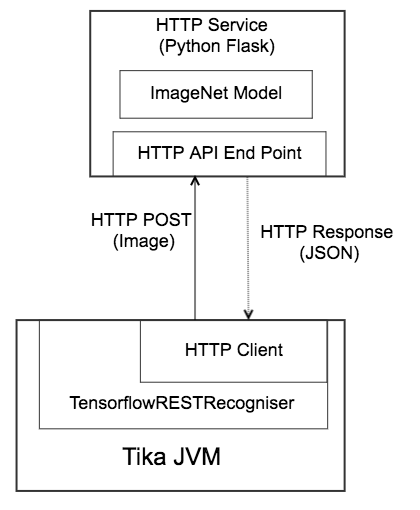
\includegraphics[scale=0.40]{tika-tflow-rest-design}

\section {EVALUATION} \label{sec:evaluation}

\subsection{Analysis of results}
\begin{figure}[h]
	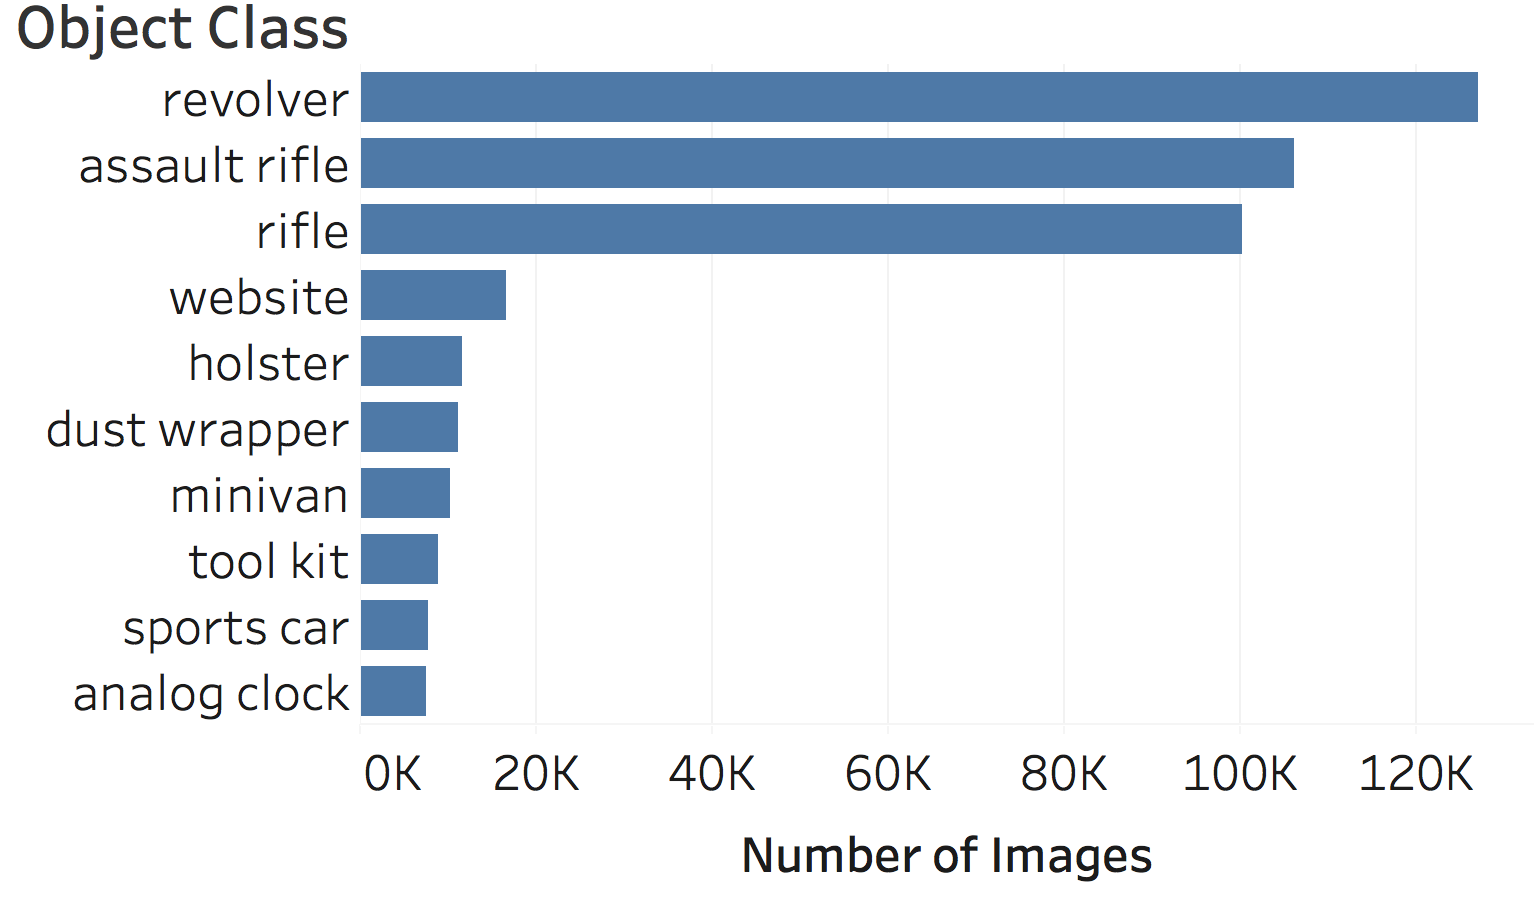
\includegraphics[width=\columnwidth]{top10classes2}
	\caption{Top 10 image classes found in the image dataset. As labeled are generated for weapon images, we can train a more targeted domain-specific classifier.}
	\label{fig:top10ImgClass}
\end{figure}
The image classifier model used in our experiments was Inception-V3 \cite{SzegedyVISW15}. The Inception-V3 model has trained on ImageNet 2012 dataset which contains 1000 classes\cite{ILSVRC15}.
The 10 most frequently occurred classes and their frequencies are shown in the Figure \ref{fig:top10ImgClass}. Since the crawlers were focused on retrieving the web pages and linked images that are related to weapons classifieds, the top classes in our dataset were found to be `revolver', and `rifle'

\subsection{Manual cross validation of results}
We cross-validated the predictions by using a subset of human-labeled images. The results are shown in Figure \ref{fig:uk-hack-eval}. 
%//TODO: Describe more if space permits
\begin{figure}[h]
	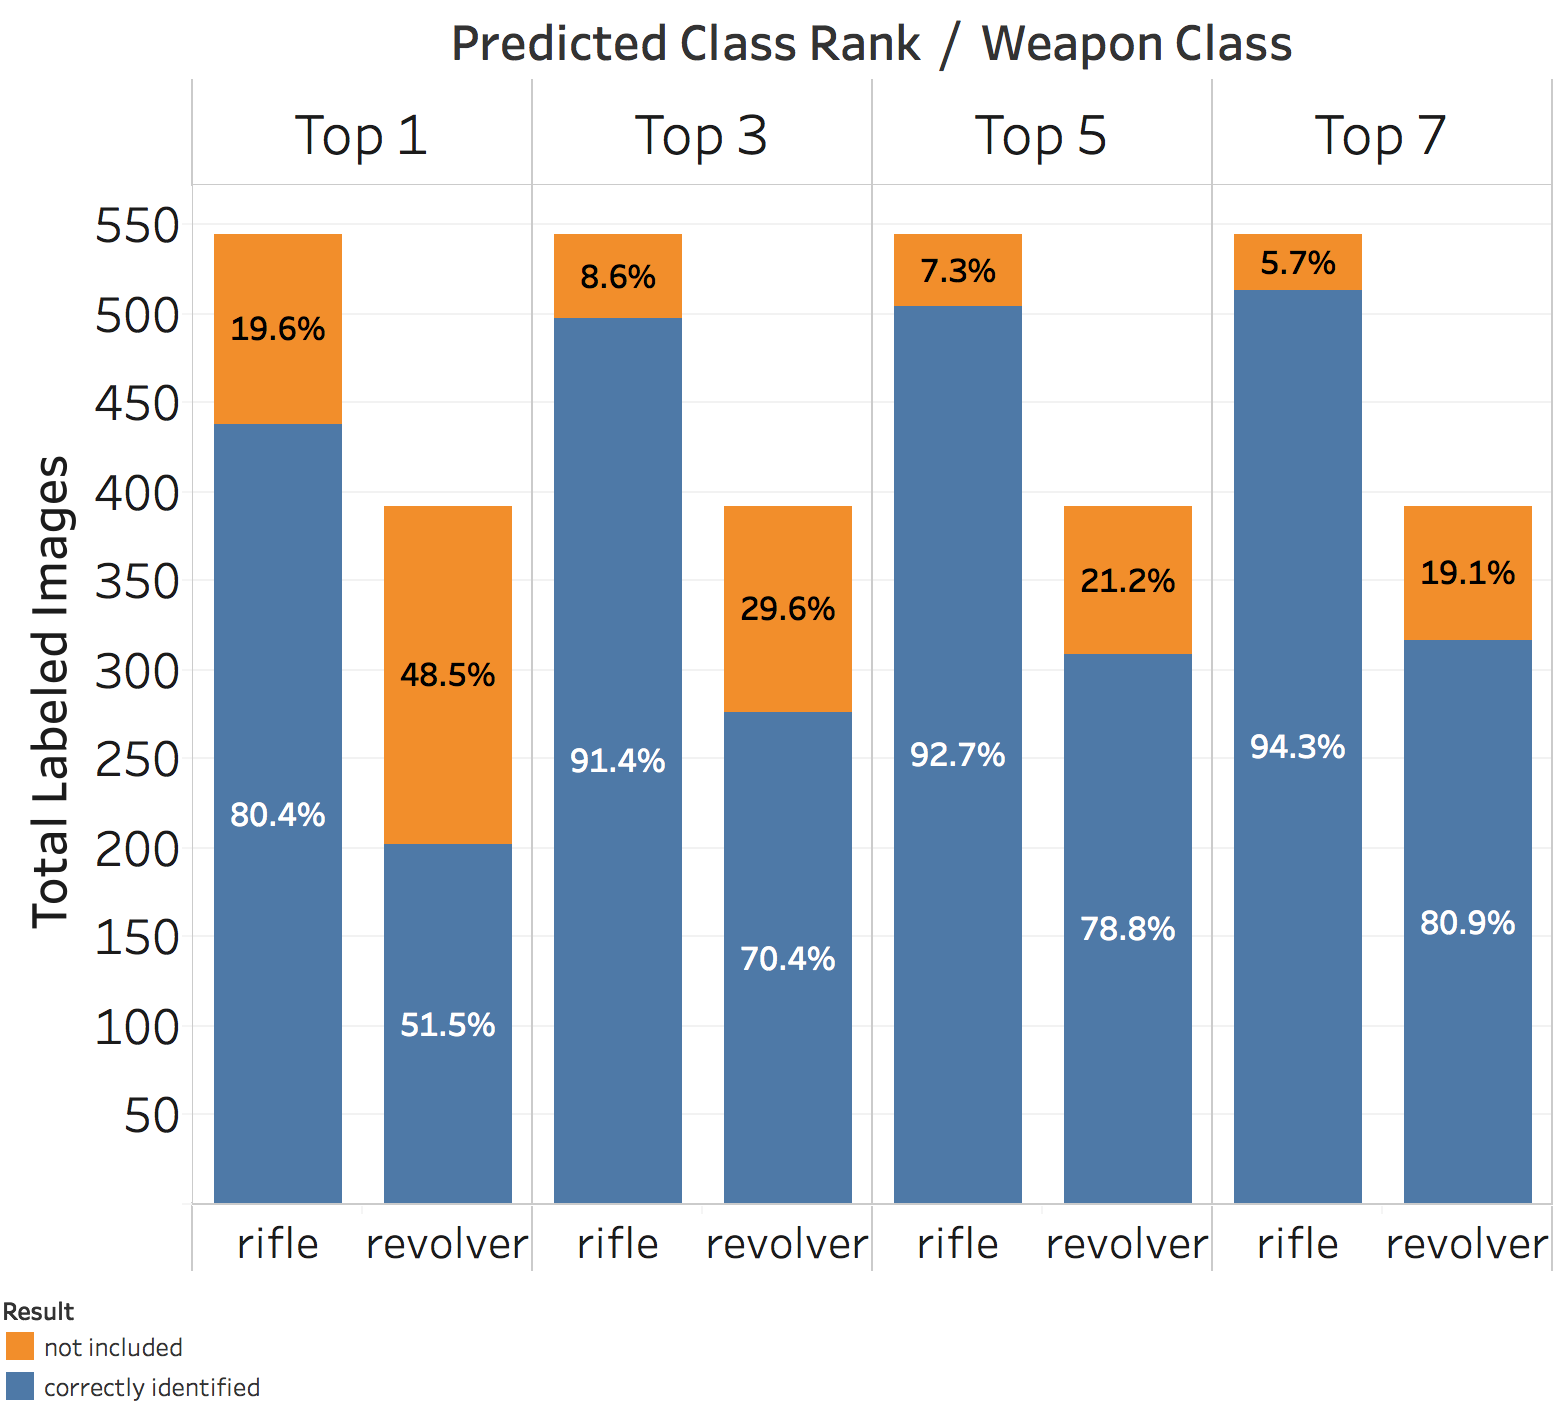
\includegraphics[width=\columnwidth]{uk-hack-evaluation3}
	\caption{Manual cross validation of results for the two weapon types: `revolver' and `rifle.' For all images, either rifle or revolver should have been the top object class identified. There is a significant portion of images where the weapon objects were identified but weren't the primary class.}
	\label{fig:uk-hack-eval}
\end{figure}

\subsection{Integration techniques}
The pros and cons of all the integration techniques described in Section \ref{sec:integration} are shown in Table \ref{tab:int-technique}.
\begin{table*}[bt]
	\centering
	\begin{tabularx}{\textwidth}{
			|p{\dimexpr.08\linewidth-2\tabcolsep-1.3333\arrayrulewidth}% column 1
			|p{\dimexpr.06\linewidth-2\tabcolsep-1.3333\arrayrulewidth}% column 1
			|p{\dimexpr.43\linewidth-2\tabcolsep-1.3333\arrayrulewidth}% column 2
			|p{\dimexpr.43\linewidth-2\tabcolsep-1.3333\arrayrulewidth}|% column 3
		} \hline

		\textbf{Method} & \textbf{Time} & \textbf{Pros} & \textbf{Cons} \\ \hline

		\textbf{CLI} 
		& 3s&
        \rule{0pt}{2.5ex}
		\tabitem Easy to develop and test \newline
		\tabitem Easy to install dependencies \newline
		\tabitem Isolation of dependencies and concerns
		& 
        \rule{0pt}{2.5ex}
        \tabitem Additional load on secondary storage to share image data. \newline
		\tabitem An extra process is created and destroyed for each call. \newline
		\tabitem Additional IO for each call since the model file is loaded and unloaded for each process  
		\\ \hline

		\textbf{JNI} 
		& N/A
        \rule{0pt}{2.5ex}
		& \tabitem The most efficient utilization of resources. \newline 
		\tabitem No external IO required since the system is monolithic.
		& 
        \rule{0pt}{2.5ex}
		\tabitem The JNI native glue code has to be produced for all the platforms. \newline
		\tabitem Utilities like \texttt{protobuf} should also be glued with JNI because they are required for deserializing models\cite{javacpp-240}.
		\\ \hline

		\textbf{gRPC}
		& 598ms
        \rule{0pt}{2.5ex}
		& \tabitem An efficient way for integrating heterogeneous systems. \newline 
		\tabitem The client system is easily portable, the server system can also be easily portable by making use of containerization or virtualization. 
		& 
        \rule{0pt}{2.5ex}  
        \tabitem The gRPC client depended on specific versions of transitive dependencies such as HTTP Client which conflicts with existing functionality based on older HTTP Clients.
		\\ \hline
		\textbf{REST API}
		& 253ms
		&
        \rule{0pt}{2.5ex}
		\tabitem An efficient way for integrating heterogeneous systems. \newline 
		\tabitem The technology and practices are popular among developers. \newline 
		\tabitem The underlying HTTP is stable and well documented.
		& 
        \rule{0pt}{2.5ex}
        \tabitem The bandwidth consumption is higher than gRPC due to the extra HTTP headers. \newline
		\\ \hline
	\end{tabularx}
\caption{Brief comparison of integration techniques. \textnormal{The numbers in the `Time' column are the time taken per image on a ubuntu 14.04 LTS docker container running on MacBook Pro 2013 model (2.8GhZ Core i7 and SSD storage) for test images of size 1024x768 pixels.}}
\label{tab:int-technique}
\end{table*}

%%%%%%%% COMMENT BEGIN
\iffalse
\subsubsection{Command Line Invocation (CLI)} \label{sec:eval-cli}
The average time taken to recognize image in this method was 6 seconds.

The pros of Command Line Interface:
\begin{itemize}
	\item Easy to develop and test
	\item Easy to install the requirements
	\item Isolation of dependencies / concerns
\end{itemize}

The cons of this technique:
\begin{itemize}
	\item The image data is shared via secondary storage which puts additional load on the secondary storage.
	\item An independent process is created and destroyed for every parse call.
	\item The ImageNet model is loaded and unloaded for every parse call due to ephemeral nature of processes. The InceptionV3 model used in our experiments is approximately 200MB in size, thus 200MB of additional IO for each parse call.
\end{itemize}

%% 2. JNI
\subsubsection{Java Native Interface (JNI)} \label{sec:eval-jni}

The pros of this method are
\begin{itemize}
	\item The most efficient utilization of resources
	\item No external input-output required as the entire task runs in a single process.
\end{itemize}

The cons of this method are:
\begin{itemize}
	\item The JNI glue code has to be compiled and packaged for all the platforms.
	\item Utilities like \texttt{protobuf} should also be glued with JNI, because they are required for deserializing models\cite{javacpp-240}.
\end{itemize}

%% 3. RPC
\subsubsection{gRPC Remote procedure Call (gRPC)} \label{sec:eval-rpc}

The pros of this method are
\begin{itemize}
	\item An efficient way for integrating heterogeneous systems.
	\item The client system is easily portable, server system can also be easily portable by making use of containerization or virtualization.
\end{itemize}

The cons of this method are:
\begin{itemize}
	\item The gRPC client depended on specific versions of transitive dependencies such as HTTP Client which conflicts with existing functionality based on older HTTP Clients.
\end{itemize}

%% 4. REST
\subsubsection{Representational State Transfer (REST) Application Programming Interface (API)} \label{sec:eval-rest}

The average REST API call was 260 milliseconds when the client and server were in the same host (i.e., the connection via loopback interface).

The pros of this method are
\begin{itemize}
	\item An efficient and popular way for integrating heterogeneous systems.
	\item The technology and practices are popular among developer community.
	\item The underlying HTTP is stable and well documented.
\end{itemize}

The cons of this method are
\begin{itemize}
	\item The performance is slightly lower than gRPC.
	\item Slightly higher bandwidth usage due to additional metadata introduced by HTTP to the packets.
\end{itemize}
\fi  %% COMMENT END

\section{FUTURE WORK} \label{sec:future}
The object recognition results discussed in section \ref{sec:evaluation} represents one of several deep learning applications developed as part of the Memex program. Serial number identification \cite{parekh2016tesseract}, image similarity \cite{zhou2016multimedia}, and video similiarity \cite{mattmann2016scalable} approaches have proven useful in various Memex domains including weapons, human trafficking, and counterfeit electronics. However, these applications have been developed independently by various Memex performers and require significant effort and coordination to integrate in crawling and extraction pipelines built upon foundational tools like Apache Nutch and Apache Tika. With the extension of Tika's capabilities into Tensorflow and deep learning frameworks, this integration becomes easier and we plan to incorporate the aforementioned approaches into Memex's core extraction pipeline going forward. 


\section{CONCLUSION} \label{sec:future}
% The recent increase of content analysis technologies and architectures makes the systemization of such tools difficult.
We have described our approach and motivation for automatically integrating image forensics into content analysis. Our motivations stem from a large corpus of 1.4 million weapons related images from the DARPA MEMEX effort, and our goals of automatically performing image classification to determine the illegal sale of automatic weapons, and other dangerous objects on the web. We integrated the widely used Google Tensorflow toolkit, and its ImageNet/Inception v3 model with the Apache Tika framework for automated and efficient image classification and analysis. We qualitatively and quantitiatvely evaluated the feasibility of our integration and report on running the integration over the MEMEX weapons data. We also describe our process for integrating Tensorflow and Tika. 


% \section{CONCLUSIONS}
%% TODO: link to Wiki page

\section*{ACKNOWLEDGMENT}
This work was supported by the DARPA XDATA/Memex program. In addition, the NSF Polar Cyberinfrastructure award numbers PLR-1348450 and PLR-144562 funded a portion of the work. Effort supported in part by JPL, managed by the California Institute of Technology on behalf of NASA.

\bibliographystyle{ACM-Reference-Format}
\bibliography{MFSEC17.bib} 

\end{document}
